\documentclass[letterpaper,10pt]{article}

%\setlength{\parindent}{0in}
%\usepackage{fullpage} 
\usepackage{amsmath}
\usepackage{amssymb}
\usepackage{enumerate}
\usepackage{graphicx}
\usepackage{color}
\usepackage[table]{xcolor}
\usepackage{dcolumn}
\oddsidemargin 0.0in
\textwidth 6.5in
\newcolumntype{.}{D{.}{.}{-1}}
\newcommand*{\myalign}[2]{\multicolumn{1}{#1}{#2}}

% Project Assignment 5 Tradeoff and System Selection is due 3/9/12. It is a team 
% event. Please see the Project area in Sakai for more guidance.
% a) Use the CAIV process to determine the non-dominated variant(s) from a plot 
% the OMOE vs. LCC and OMOE vs. TOC. Identify each variant as either 
% dominated or non-dominated.
% b) Evaluate the results considering the sensitivity of the two most important 
% KPPs (based on attribute weights) on the overall selection of a best variant.
% c) Recommend variant characteristics for development of a future variant, and 
% identify your best variant from among the options provided.
% d) Summarize the findings with respect to the concept CAIV trade-off outcomes 
% on CAIV plots, and make a final recommendation as to the overall IED system 
% development.

\title{Project 5 \\ \Large Team CLEAR \\ \normalsize (\textcolor{red}{C}onvoy \textcolor{red}{L}evel \textcolor{red}{E}xplosive \textcolor{red}{A}mmunition \textcolor{red}{R}emoval)}
\author{Christian Aall: Testing \& Evaluation \\ 
	Steve Mazza: Team Lead \\ 
	Michael Oexmann: Analyst \\ 
	Elizabeth Swisher: Lead Systems Engineer}
	
\date{March 9, 2012}

\begin{document}
\maketitle
\tableofcontents
\listoftables
\listoffigures
\pagebreak

\section{Identification of Variants}
Following the Cost As an Independent Variable (CAIV) method, plots of the Overall Measures of Effectiveness (OMOEs) vs. Scaled Life Cycle Cost (LCC) and OMOE vs. Scaled Total Ownership Cost (TOC), were generated to compare the robot variants. These graphs can be seen in Figure \ref{fig:CAIV1} on page \pageref{fig:CAIV1} and Figure \ref{fig:CAIV2} on page \pageref{fig:CAIV2} respectively. 

\begin{figure}[h!tbp]
	\begin{center}
		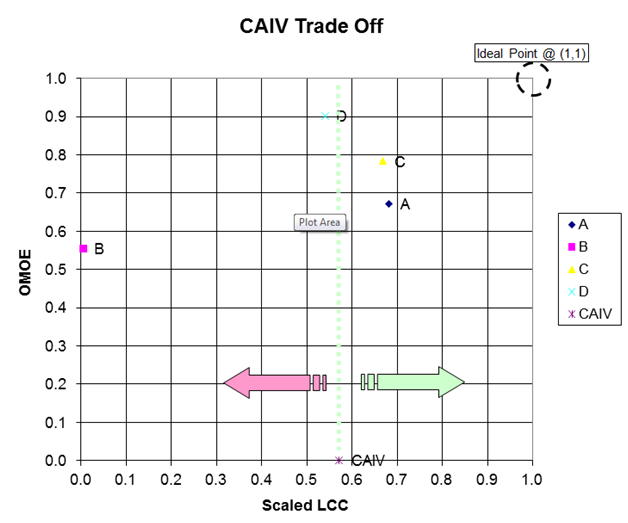
\includegraphics[scale=0.65]{images/CAIV1.png}
	\end{center}
	\caption{CAIV analysis of discounted, scaled LCC of variants A, B, C and D}
	\label{fig:CAIV1}
\end{figure}

\begin{figure}[h!tbp]
	\begin{center}
		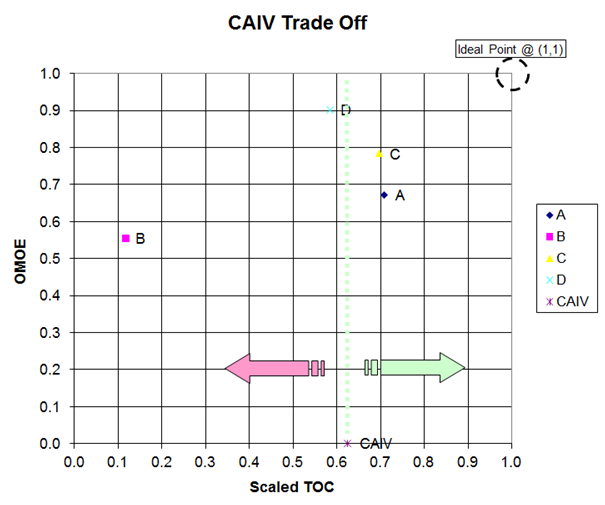
\includegraphics[scale=0.65]{images/CAIV2.png}
	\end{center}
	\caption{CAIV analysis of discounted, scaled TOC of variants A, B, C and D}
	\label{fig:CAIV2}
\end{figure}

By analyzing these plots, a determination of the optimal overall variant, based on OMOEs and cost can be identified. Based on the results, variant $C$ is best variant as it is closest to the \emph{ideal point} and furthest from the \emph{non-ideal point}. Variants $A$, $C$, and $D$, were all determined to be \emph{non-dominated} variants due to their proximity to the ideal point and relative proximity to the Pareto curve boundaries. Variant $B$ was considered to be dominated due to its location on the graph and distance with regard to the ideal and non-ideal solution points.

\section{Evaluation}
At the request of the DoD, we analyzed variants for sensitivity to weighting of KPPs.  The two highest weighted KPPs from our study were Mission Reliability and Operational Availability with weights of 0.248 and 0.289 respectively. The two KPPs in question by the DoD for bias are Mission Reliability and DRM Elapsed Time, which were weighted at 0.064. Despite having our heaviest weight we first studied if Mission Reliability was still underweight. The table below (see Table \ref{tab:MissionReliability} on page \pageref{tab:MissionReliability}) shows the results of all four variants by comparing the Mission Reliability weight from our study to the extreme case where Mission Reliability has a weight of 1. The results were then graphed using a trend line to show weightings between those values (see Figure \ref{fig:MissionReliability} on page \pageref{fig:MissionReliability}).

\begin{table}[h!tbp]\footnotesize
	\begin{center}
		\begin{tabular}{l........}
		\hline
		& \multicolumn{2}{c}{\textbf{A}}
		& \multicolumn{2}{c}{\textbf{B}}
		& \multicolumn{2}{c}{\textbf{C}}
		& \multicolumn{2}{c}{\textbf{D}} \\
		& \myalign{c}{Original} 
		& \myalign{c}{Weight=1} 
		& \myalign{c}{Original} 
		& \myalign{c}{Weight=1} 
		& \myalign{c}{Original} 
		& \myalign{c}{Weight=1} 
		& \myalign{c}{Original} 
		& \myalign{c}{Weight=1} \\
		\hline\hline
		\textbf{Weight} & 0.248 & 1 & 0.248 & 1 & 0.248 & 1 & 0.248 & 1 \\
		\textbf{Total Score} & 0.672 & 0.400 & 0.554 & 0.800 & 0.784 & 0.800 & 0.901 & 1.000 \\
		\hline
		\end{tabular}
	\end{center}
	\caption{Mission Reliability}
	\label{tab:MissionReliability}
\end{table}

\begin{figure}[h!tbp]
	\begin{center}
		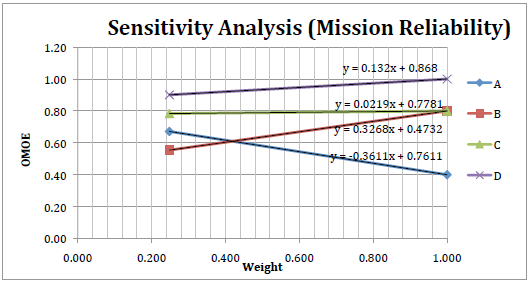
\includegraphics[scale=0.65]{images/MissionReliability.png}
	\end{center}
	\caption{Mission Reliability}
	\label{fig:MissionReliability}
\end{figure}

Variant $D$ still maintained the top score for OMOE under all weights tested by the trend line. Increasing the weighting of Mission Reliability had minimal effect on Variant $C$'s OMOE. Increasing Mission Reliability weight had a noticeable positive effect on the OMOE for variant $B$ but it was only able to match but not overtake variant $C$ in the most extreme case of a weighting of 1. Since Variant $B$ has the highest cost it is still dominated. Variant $A$ was downgraded significantly by an increase of weighting of Mission Reliability and overtaken in OMOE by variant $B$ at approximately a weighting of 0.42. After further analysis we are confident in our proposed weighting of Mission Reliability and are confident our results were not skewed by potentially under weighting its importance. 

DRM Elapsed Time was also studied in greater detail. The Table \ref{tab:DRMElapsedTime} on page \pageref{tab:DRMElapsedTime} shows the results of all four variants by comparing the DRM Elapsed Time weight from our study to the extreme case where DRM Elapsed Time has a weight of 1. The results were then graphed using a trend line to show weightings between those values.

\begin{table}[h!tbp]\footnotesize
	\begin{center}
		\begin{tabular}{l........}
		\hline
		& \multicolumn{2}{c}{\textbf{A}}
		& \multicolumn{2}{c}{\textbf{B}}
		& \multicolumn{2}{c}{\textbf{C}}
		& \multicolumn{2}{c}{\textbf{D}} \\
		& \myalign{c}{Original} 
		& \myalign{c}{Weight=1} 
		& \myalign{c}{Original} 
		& \myalign{c}{Weight=1} 
		& \myalign{c}{Original} 
		& \myalign{c}{Weight=1} 
		& \myalign{c}{Original} 
		& \myalign{c}{Weight=1} \\
		\hline\hline
		\textbf{Weight} & 0.064 & 1 & 0.064 & 1 & 0.064 & 1 & 0.064 & 1 \\
		\textbf{Total Score} & 0.672 & 0.390 & 0.554 & 0.660 & 0.784 & 0.180 & 0.901 & 0.870 \\
		\hline
		\end{tabular}
	\end{center}
	\caption{DRM Elapsed Time}
	\label{tab:DRMElapsedTime}
\end{table}

\begin{figure}[h!tbp]
	\begin{center}
		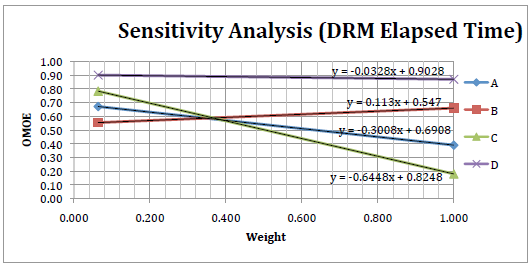
\includegraphics[scale=0.65]{images/DRMElapsedTime.png}
	\end{center}
	\caption{DRM Elapsed Time}
	\label{fig:DRMElapsedTime}
\end{figure}

After adjusting DRM Elapsed Time weight, variant $D$ once again maintained the top OMOE score with only a slight small downgrade in OMOE from 0.901 at a weight of 0.064 to an OMOE of 0.87 with a weight of 1. Interestingly variants $A$, $B$, and $C$ all merge in OMOE score at weighted approximately 0.36 - 0.38 for DRM Elapsed Time.  After that weight range, variant $B$ is able to move from the worst performer to being superior to both variant $A$ and $C$. Variant $B$ is still dominated by variant $D$ due to its high cost. Although both variant $A$ and $C$ suffer declines in OMOE as the weighting of DRM Elapsed Time increases, variant $A$ passes variant $C$ in performance at approximately a weighting of 0.38.

Increasing the DRM Elapsed Time does shed an interesting light on overall findings.  Variant $B$ remains dominated. Variant $D$ still offers the best performance is the price is acceptable and looks more impressive in comparison to Variants $A$ and $C$ as the weighting of DRM Elapsed Time increases. DRM Elapsed Time would need to become the heaviest weighted attribute in order to dominate variant $C$, a proposal we do not agree with. Variant $A$ remains an acceptable alternative if the cost of variants $C$ and $D$ are prohibitive. Variant $C$ suffers a drastic decline in performance as DRM Elapsed Time increases in weight but under weighting where DRM Elapsed Time is not considered the most important KPP is still a good choice.

\section{Recommendations}
The assessment above indicates that variant $A$, $C$, and $D$ have the most desirable cost to performance characteristics. In the CAIV analysis, the team established a means of graphically depicting the lowest performing variant when compared to other options, while simultaneously comparing the life cycle cost and total ownership cost of the proposed variant. Through the means of a Pareto curve assessment, it was discovered that variant $A$, $C$ and $D$ fell within the non-dominated region, while variant $B$ resided within the dominated region. Additionally, two out of the three non-dominated variants ($A$ and $C$) exceeded the CAIV threshold and therefore indicated strongest performance for the given life-cycle cost. Furthermore, an assessment of the Euclidean distance of the respective variants from the most ideal cost and performance values indicated that variant $C$ was most desirable in terms of CAIV.

The sensitivity assessment indicated that variant $D$ still maintained highest scores for OMOEs under all weights tested by the trend line. Increasing weights of the highest priority OMOEs (Mission Reliability and DRM Elapsed Time) indicated that variants $A$ and $C$ may score lower than variants $B$ and $D$ in these OMOEs. This assessment also indicated that variant $D$ will continue to offer the best performance, even if weights for highest priority OMOEs were increased.

Team CLEAR feels that further improvements made to the SMETAL-V system may improve high priority OMOE performance and provide for a more desirable end item. To increase Mission Reliability, team CLEAR recommends water tight electrical connections and hardened (drive) track links to ensure continued operation in all environments. Additionally, to improve the DRM elapsed time, higher speed drive trains, faster computing hardware, and higher sensitivity sensor system should be implemented. 

\section{Summary}
After thorough analysis of weighted performance measures, costs, risk, and sensitivity for variants $A$, $B$, $C$, and $D$, CLEAR recommends that further developmental activities and spending be focused on variant $D$. Variant $D$, though not the best performing regarding CAIV, has performed significantly better in almost all OMOEs, while exhibiting reasonable life-cycle costs, total ownership costs, and low risk. Its consistency in all testing and evaluation of OMOEs indicates that it exhibits stability and predictability in most aspects of operation. This will allow for maintenance and support activities to be performed at known intervals with little volatility in \emph{up-time} and \emph{down-time}. The logistics and support chain will be constant, with a low chance of emergency repairs due to unpredictable performance.

\end{document}
